\documentclass[11pt,openany]{memoir}
\usepackage[usenames,dvipsnames]{xcolor}
\usepackage{amssymb}
\usepackage{amsmath}
\usepackage{amsthm}
\usepackage{url}
\usepackage{xspace}
\usepackage[margin=2.5cm]{geometry}
\usepackage{tikz}
\usetikzlibrary{positioning,calc,matrix,arrows}
\usepackage{pgfplots}
\usepackage{listings}
\usepackage{color}
\usepackage{textcomp}
\usepackage{fancyvrb}
\usepackage{array}
\usepackage{dirtytalk}
\usepackage[colorlinks]{hyperref}
\usepackage{cleveref}

% NOTE: This template is based on the MatConvNet manual written by Andrea Vedaldi, Karel Lenc and Ankush Gupta.

\newtheorem{example}{Example}
\newtheorem{lemma}{Lemma}

\newcommand{\real}{\mathbb{R}}
\newcommand{\xx}{\mathbf{x}}
\newcommand{\yy}{\mathbf{y}}
\newcommand{\pp}{\mathbf{p}}
\newcommand{\hh}{\mathbf{h}}
\newcommand{\diag}{\operatorname{diag}}
\newcommand{\bone}{\mathbf{1}}
\newcommand{\FF}{\mathcal{F}}
\newcommand{\ththeta}{\pmb{\theta}}
\newcommand{\EE}{\mathbb{E}}
\DeclareMathOperator{\dd}{\text{d}}
\newcommand{\vv}{\operatorname{vec}}
\newcommand{\tr}{\operatorname{tr}}
%\newcommand{\matconvnet}{\textsc{MatConvNet}\xspace}
%\newcommand{\matlab}{\textsc{MATLAB}\xspace}
%\newcommand{\cpp}{C{}\texttt{++}~}
%\newcommand{\by}{\mathbf{y}}
%\newcommand{\bc}{\mathbf{c}}
%\newcommand{\bz}{\mathbf{z}}
%\newcommand{\bff}{\mathbf{f}}
%\newcommand{\bg}{\mathbf{g}}
%\newcommand{\br}{\mathbf{r}}
%\newcommand{\bw}{\mathbf{w}}
%\newcommand{\bp}{\mathbf{p}}
%\newcommand{\bfs}{\mathbf{s}}
%\newcommand{\bfe}{\mathbf{e}}
\newcommand{\samsays}[1]{\textcolor{RubineRed}{[S: #1]}}

%\newcommand{\argmin}{\operatornamewithlimits{argmin}}
%\newcommand{\argmax}{\operatornamewithlimits{argmax}}
%\newcommand{\sign}{\operatornamewithlimits{sign}}
%
%\tikzstyle{block} = [draw, rectangle, minimum height=3em, minimum width=3em]
%\tikzstyle{data} = []
%\tikzstyle{datac} = [draw, circle, minimum height=2.5em, minimum width=2.5em,inner sep=3pt,font=\footnotesize]
%\tikzstyle{par} = [draw, circle, minimum height=2.5em, minimum width=2.5em,fill=black!20,inner sep=3pt,font=\footnotesize]
%\tikzstyle{pinstyle} = [pin edge={to-,thin,black}]
%\tikzstyle{to} = [->,>=stealth',shorten >=1pt,semithick]
%\tikzstyle{from} = [<-,>=stealth',shorten >=1pt,semithick]
%\tikzstyle{bp} = [draw=blue,text=blue]
%\tikzstyle{bpl} = [draw=blue!40]
%\tikzstyle{bpe} = [text=blue,draw=none]

\VerbatimFootnotes

\setsecnumdepth{subsection}
\settocdepth{subsection}

\definecolor{listinggray}{gray}{0.9}
\definecolor{lbcolor}{rgb}{0.8,0.8,0.8}
\lstset{
	%backgroundcolor=\color{lbcolor},
	tabsize=4,
	rulecolor=,
	language=matlab,
	basicstyle=\small,
	upquote=true,
	columns=fullflexible,
	showstringspaces=false,
	extendedchars=true,
	breaklines=false,
	prebreak = \raisebox{0ex}[0ex][0ex]{\ensuremath{\hookleftarrow}},
	%frame=single,
	showtabs=false,
	showspaces=false,
	showstringspaces=false,
	identifierstyle=\ttfamily,
	keywordstyle=\color[rgb]{0,0,1},
	commentstyle=\itshape\color[rgb]{0.133,0.545,0.133},
	stringstyle=\color[rgb]{0.627,0.126,0.941},
}
\lstMakeShortInline[columns=fullflexible, breaklines = true,
 breakatwhitespace = true]!

\title{Differentials for Applied Computer Vision}
\author{
Samuel Albanie
}
\date{}

\hypersetup{
  pdfinfo={
    Title={Differentials for Applied Computer Vision},
    Author={Samuel Albanie},
		Subject={Notes on Mathematics},
    Keywords={computer vision, differentials, machine learning}
  }
}

\sloppy

% ------------------------------------------------------------------
\begin{document}
% ------------------------------------------------------------------

%\end{document}

\frontmatter
\maketitle{}

\begin{abstract}
The purpose of this short note is to collect together a set of useful
calculus derivations using the framework of \textit{matrix differentials}. The goal is to develop it over time and therefore it should be considered a work-in-progress.  Consequently any contributions, feedback or notifications of mistakes are much appreciated\footnote{Feel free to contact me by raising an issue on the github page, submitting a pull request directly (\mbox{\url{https://github.com/albanie/derivations})}}).
\end{abstract}
\clearpage

\tableofcontents*
\clearpage

\mainmatter
\chapter{Introduction}\label{sec:intro}

Calculus plays a central role in computer vision. As the community has integrated ever more closely with techniques from machine learning, statistics and optimisation, the ability to differentiate vector and matrix functions has become more useful to computer vision researchers.  Unfortunately, multivariate calculus, when performed with indices over element locations is a fairly tricky business to build an intuition for.  Although the index-based approach has the majority of the market share in the research world, there is an alternative: the slightly lesser known method of \textit{matrix differentials}.  We have found this alternative approach to be significantly simpler, more intuitive and faster to work with.  

Finally, we note that the widespread adoption of automatic differentiation (autodiff) has been a major boon to the whole community, in many cases obviating the need to perform arduous pen and paper derivations.  The goal of these notes is not to encourage the reader to avoid using autodiff, but to assist them in understanding, on a mathematical level, what is going on \say{under the hood}.


\section{Useful Resources}

There are a number of extremely good references for getting to grips with the calculus of vector and matrix functions.  Below are a few that we have found particularly useful, providing much of the material for these notes:

\begin{itemize}
\item Written by econometricians Magnus and Neudecker (originally in $1988$, but revised several times), \textit{Matrix differential calculus with applications in statistics and econometrics} is the canonical reference for matrix differential calculus~\cite{magnus1988matrix}.
\item The fundamentals of working with matrices \cite{searle2017matrix}.
\item \cite{kinghorn1996integrals}, \cite{minka2000old} and \cite{petersen2008matrix} each contain a large number of highly useful results and are good as quick references.
\item The MatConvNet manual \cite{vedaldi2015matconvnetmanual} provides carefully worked through examples of matrix derivatives.  While the emphasis is primarily on index-based derivations, it provides the derivatives of many common neural network computation blocks in matrix form and is very useful as a reference. 
\end{itemize}
\chapter{Vector Functions} \label{chap:vector}

\section{Element-wise operators}

Often, we are tasked we computing the gradient of a function $\phi: \real^n \to \real^n$ that takes the form of an \textit{element-wise operator}.  By this, we mean that there exists some scalar function $f:\real \to \real$ such that for any $\xx \in \real^n$

\begin{align}
  [\phi(\xx)]_i = f(\xx_i), \quad \forall i \in \{1, \dots, n\}
\end{align}

For these operators, it is helpful to first compute the derivative of the scalar component function,~$f'$.  This can then be used in combination with differentials to compute the gradient of $\phi$ as follows:

\begin{align}
  \underbrace{{\dd}\phi(\xx)}_{n \times 1} = \underbrace{\diag(f'[\xx])}_{n \times n} \underbrace{\vphantom{(}{\dd
}\xx}_{n \times 1} \label{eqn:eltwise-differentials}
\end{align}

where we have used the notation $f'[\xx]$ to denote that $f'$ is applied element-wise to each element of $\xx$ (this notation is used throughout the document), and the dimensions of each term are displayed beneath the equation. 


\section{Sigmoid}

The sigmoid function is often used as an elementwise operator in neural networks.  The sigmoid is a scalar map $\sigma : \real \to \real$ defined by: 

\begin{align}
\sigma (x) = \frac{1}{1 + e^{-x}} = \frac{e^x}{1 + e^x}  
\end{align}


We can compute its gradients using the quotient rule:

\begin{align*}
  \dd (\sigma(x)) &= {\dd} \bigg(\frac{e^x}{1 + e^x}\bigg) \\
                  &= \frac{(1 + e^x) \dd (e^x) - e^x \dd (1 + e^x)}{(1 + e^x)^2}
               = \frac{(1 + e^x)e^x \dd x - e^x e^x \dd x}{(1 + e^x)^2} \\
               &= \Bigg(\frac{e^x((1 + e^x) - e^x)}{(1 + e^x)^2}\Bigg)\dd x = \Bigg(\frac{e^x}{(1 + e^x)}\frac{1}{(1 + e^x)}\Bigg){\dd} x \\
               &= \sigma(x)(1 - \sigma(x)) {\dd} x \\                              
\end{align*}

which tells us that $\sigma'(x) = \sigma(x) (1 - \sigma(x))$.  The sigmoid and its derivative are shown in Fig.\ref{fig:sigmoid}.  We can now apply Eqn.\ref{eqn:eltwise-differentials} to obtain the Jacobian of the element-wise sigmoid:

\begin{align}
\dd (\sigma[\xx]) = \diag\Big(\sigma[\xx]\circ(\bone - \sigma[\xx])\Big){\dd} \xx
\end{align}

Since the diagonal matrix is symmetric, it follows that $\nabla \sigma(\xx) = \diag\Big(\sigma[\xx]\circ(\bone - \sigma[\xx])\Big)$.

\begin{figure}
\centering
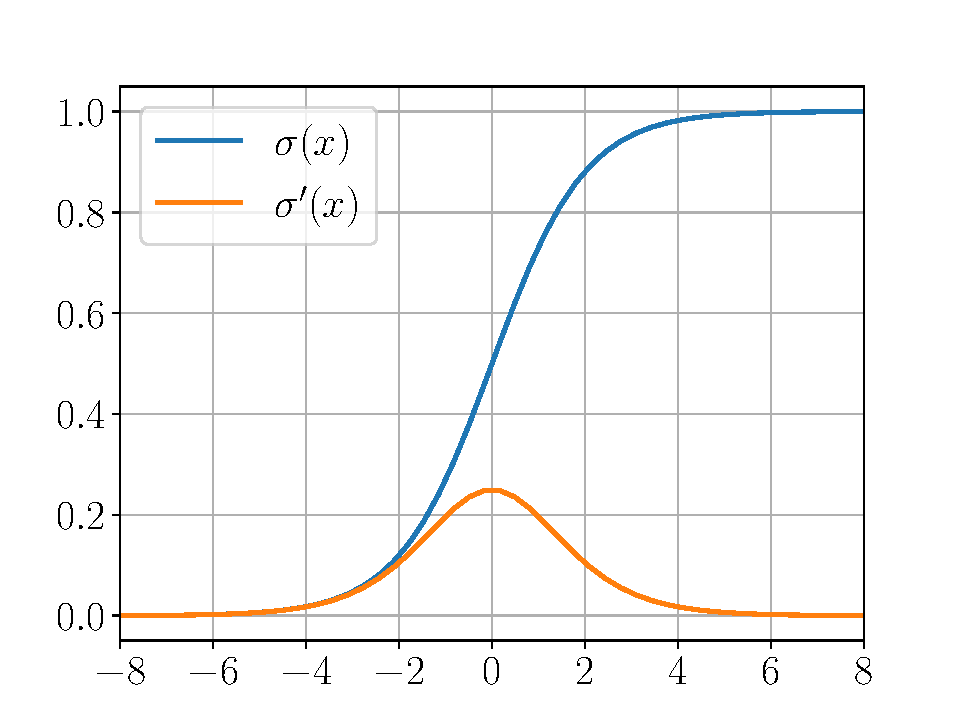
\includegraphics[width=0.5\textwidth]{figs/sigmoid.pdf}
\caption{The sigmoid function and its derivative.\label{fig:sigmoid}}  
\end{figure}

\section{Softmax} \label{sec:softmax}

The softmax function represents another vector function that is commonly used as a computational block in neural networks.  It can be viewed as a form of generalised sigmoid (for this reason it is common to overload the $\sigma$ symbol for the softmax, $\sigma : \real^n \to \real^n$).  It may be helpful to keep in mind that although it produces an output with the same shape as its input, it is not an element-wise operator and $\sigma(\xx) \neq \sigma[\xx]$ (i.e. it does not produce the same output as an element-wise sigmoid).  It is defined by:

\begin{align}
\sigma (\xx) = \frac{\exp[\xx]}{\bone^T \exp[\xx]} 
\end{align}

Note that the denominator here is a scalar, while the numerator has shape $n \times 1$.  To compute the gradient of this function, we can proceed with differentials:

\begin{align}
  \dd(\sigma(\xx)) &= \dd \Bigg( \frac{\exp[\xx]}{\bone^T \exp[\xx]} \Bigg) \\
                 &= \frac{(\bone^T \exp[\xx]) \dd (\exp[\xx]) - \exp[\xx] \dd (\bone^T \exp[\xx])}{(\bone^T \exp[\xx])(\bone^T \exp[\xx])} \\
                 &= \frac{(\bone^T \exp[\xx]) \diag(\exp[\xx]){\dd} \xx - \exp[\xx] (\bone^T \diag(\exp[\xx]){\dd}\xx)}{(\bone^T \exp[\xx])(\bone^T \exp[\xx])} && \text{(using \ref{eqn:eltwise-differentials})}\\
                 &= \Bigg(\frac{\diag(\exp[\xx])}{(\bone^T \exp[\xx])} - \frac{\exp[\xx] (\bone^T \diag(\exp[\xx]))}{(\bone^T \exp[\xx])(\bone^T \exp[\xx])}\Bigg){\dd}\xx \\
                  &= \Bigg(\diag(\sigma(\xx)) - \sigma(\xx)\sigma(\xx)^T\Bigg){\dd}\xx && \text{(using \ref{eqn:diagLinear})} \label{eqn:vectorSoftmax}
\end{align}

Since both terms are symmetric matrices, it follows that $\nabla\sigma(\xx) = \diag(\sigma(\xx)) - \sigma(\xx)\sigma(\xx)^T$.  

There are also often cases where we would like to apply the softmax operator to a higher order tensor.  The simplest way to address this notationally is define the softmax operator $\sigma(\cdot)$ to always act along the first non-singleton dimension. Thus for an $m \times n$ matrix $X = [\xx_1 | \dots | \xx_n]$ (with each $\xx_i \in \real^m$), the action of the softmax operator produces the following effect:

\begin{align*}
  \sigma(X) &= \sigma \Big( \left[\begin{array}{c|c|c}
  \xx_1 & \dots & \xx_n
\end{array}\right] \Big) \\
 &= \left[\begin{array}{c|c|c}
  \sigma(\xx_1) & \dots & \sigma(\xx_n)
\end{array}\right]
\end{align*}

We can derive the gradient of this operator with respect to an input matrix $X \in \real^{m \times n}$, using the vec operator. This is a little more involved than the previous derivations, so the equations are interspersed with visualisations.  The overall strategy is to reach an expression of the form $\dd \vv(\sigma(X)) = A \dd \vv(X)$ and apply the identification theorem \citep{magnus1988matrix} to read off the Jacobian of the softmax as $A \in \real^{mn \times mn}$.

\begin{align}
  \dd(\vv(\sigma(X))) &= \dd \big( \left[\begin{array}{c}
  \sigma(\xx_1) \\
  \vdots \\
  \sigma(\xx_n)
\end{array}\right] \big) =
\left[\begin{array}{c|c|c}
  \dd (\sigma(\xx_1); \xx_1) & \hdots & {\dd} \sigma(\xx_1; \xx_n) \\
  \hline
  \vdots & \ddots & \vdots \\
  \hline  
  \dd (\sigma(\xx_n); \xx_1) & \hdots & \dd(\sigma(\xx_n); \xx_n) \\
\end{array}\right] \label{eqn:matrixSoftmax}
\end{align}

Here, we are writing the differential operator $\dd(\cdot ; \cdot)$ with an explicit dependence on its increment as the second argument (i.e. as defined in Eqn.~\ref{eqn:vecDifferential}), rather than leaving this to be determined implicitly as was done previously.  The off-diagonal terms disappear so we are left with the block diagonal matrix $A$ where block $ii$ contains $\dd(\sigma(\xx_i); \xx_i)$ i.e. the vector differential of the softmax. 

We therefore see that the $\sigma(\cdot)$ operator has several different meanings depending on the shape of its input (e.g. sigmoid, standard vector softmax, column-wise softmax for scalars, vectors and matrices respectively). Thus we can replace the last term in Eqn.~\ref{eqn:matrixSoftmax} with the differentials found in Eqn.~\ref{eqn:vectorSoftmax} to proceed:

\begin{align}
= \left[\begin{array}{c|c|c}
  \diag(\sigma(\xx_1)) - \sigma(\xx_1)\sigma(\xx_1)^T \dd \xx_1 & \hdots & 0_m \\
  \hline
  \vdots & \ddots & \vdots \\
  \hline  
  0_m & \hdots & \diag(\sigma(\xx_n)) - \sigma(\xx_n)\sigma(\xx_n)^T \dd \xx_n \\
\end{array}\right]  
\end{align}

where $0_m$ denotes an $m \times m$ matrix of zeros. We can summarise this a little more concisely as follows:

\begin{align}
  \dd(\vv(\sigma(X))) = \Bigg(\diag(\sigma(X)) - (I_n \otimes \underbrace{\bone \bone^T}_{m \times m}) \circ (\sigma(X)\sigma(X)^T)\Bigg) {\dd}\vv(X) \label{eqn:matrixSoftmaxDiff}
\end{align}

We see that the resulting Jacobian closely mirrors that of the vector function derived in Eqn.~\ref{eqn:vectorSoftmax}, except that there is an additional block matrix of ones that prevents enforces that partial derivatives are zero between elements in the outputs of one column and elements in the inputs from different columns.

\chapter{Loss Functions} \label{chap:loss-functions}

Loss functions are scalar functions that commonly require derivatives. 

\section{Cross Entropy}

Cross entropy measures the distance between two distributions by computing the average number bits required to encode symbols drawn from one distribution using the optimal coding scheme of the other. Given discrete distributions, $p$ and $q$, we define the cross entropy between them as:

\begin{align}
  H[p,q] &= -\sum_{\xx} p(\xx) \log q(\xx) = -\EE_{\xx \sim p} \log q(\xx) \label{eqn:cross-ent}\\
         &= \underbrace{-\sum_{\xx} p(\xx) \log p(\xx)}_{H[p]} + \underbrace{\sum_{\xx} p(\xx) \log\frac{p(\xx)}{q(\xx)}}_{\text{D}_\text{KL}(p || q)}
\end{align}

In the machine learning context, we typically cannot evaluate Eqn.\ref{eqn:cross-ent} across the full distribution $p(\xx)$.  Instead, we often have some number (e.g. $m$) of samples, $m$, and the respective probability of each sample under $p$ (the ground truth) and $q$ (the predictions we are trying to match against the ground truth). Stacking the probabilities into vectors $\mathbf{\hat{p}}, \mathbf{\hat{q}} \in \real^m$, we can rewrite Eqn.\ref{eqn:cross-ent} as the loss corresponding to $m$ samples as $\mathbf{\hat{p}}^T \log [\mathbf{\hat{q}}]$ (here we have made use of the element-wise $\log[\cdot]$ operator notation).  As before, we compute differentials:

\begin{align*}
\dd H = \dd (\mathbf{\hat{p}}^T \log [\mathbf{\hat{q}}]) = \underbrace{\mathbf{\hat{p}}^T}_{1\times n} \underbrace{\diag(\mathbf{\hat{q}})^{-1}}_{n \times n} \underbrace{\dd \mathbf{\hat{q}}}_{n \times 1}
\end{align*}

(where we have used Eqn.\ref{eqn:eltwise-differentials} for the last equality), so the gradient with respect to the predicted distribution across samples is $\nabla_{\mathbf{\hat{q}}} H = \diag(\mathbf{\hat{q}})^{-1} \mathbf{\hat{p}}$.

\section{Binary Logistic Regression}

Logistic regression is a common tool for learning a binary classifier (the problem setup described here is based on \cite{defreitas}).  The loss is often optimised with IRLS (Iterative Reweighted Least Squares), which requires not only the gradient, but also the hessian of the loss w.r.t the parameters.  We will perform the derivations with differentials.  Suppose that we are given $n$ training pairs $\{\xx_i, y_i\}_{i=1}^n$ consisting of observations $\xx_i \in \real^d$ and labels $y_i \in \real$, and would like to find the parameters $\pmb{\theta} \in \real^d$ that maximise the likelihood of the labels conditioned on the observations under a Bernoulli model:

\begin{align*}
  p( \yy | X, \mathbf{\theta}) = \prod_{i=1}^n \text{Ber}(y_i| \sigma(\xx_i^T \pmb{\theta}))
\end{align*}

where we have used $X$ to denote the $d \times n$ matrix formed by stacking the observations as columns and $\yy \in \real^{n} $ as a column vector formed from the labels.  Rather than maximising likelihood, we find $\ththeta$ by minimising the negative log-likelihood:

\begin{align*}
  \mathcal{L}(\ththeta) = - \sum_{i =1}^n y_i \log \sigma(\xx_i^T\ththeta) + (1 - y_i) \log (1 - \sigma(\xx_i^T \ththeta))
\end{align*}

We can rewrite this in a more convenient form, again using $[\cdot]$ element-wise operator notation:

\begin{align*}
  \mathcal{L}(\ththeta) = -\yy^T \log[\sigma[X^T\ththeta]] - (\bone - \yy)^T \log[\bone - \sigma[X^T\ththeta]]
\end{align*}

To find the gradient, let's write $\pmb{\pi} = \sigma[X^T\ththeta]$, noting that $\dd \pmb{\pi} = \diag(\pmb{\pi}\circ (\bone - \pmb{\pi}))X^T \dd \ththeta$, and take differentials:

\begin{align}
  \dd \mathcal{L} &= -\yy^T \dd(\log[\pmb{\pi}]) - (\bone - \yy)^T \dd(\log[\bone - \pmb{\pi}]) \\
                  &= -\yy^T \diag(\pmb{\pi})^{-1}\diag(\pmb{\pi} \circ ( \bone - \pmb{\pi}))X^T \dd \ththeta \nonumber \\
                  & \quad \quad - (\bone - \yy)^T \diag(\bone - \pmb{\pi})^{-1}\diag(-\pmb{\pi} \circ ( \bone - \pmb{\pi})) X^T \dd \ththeta && \text{(using \ref{eqn:eltwise-differentials})} \\
                  &= -\yy^T \diag(\bone - \pmb{\pi})X^T \dd \ththeta - (\bone - \yy)^T \diag(-\pmb{\pi}) X^T \dd \ththeta && \text{(using \ref{eqn:diagHadProd})}\\                  
                  &= \Big(-\yy^T \diag(\bone - \pmb{\pi}) + (\bone - \yy)^T \diag(\pmb{\pi})\Big) X^T \dd \ththeta\\                                    
                  &= \Big(-\yy^T (I_n - \diag(\pmb{\pi})) + (\bone - \yy)^T \diag(\pmb{\pi})\Big) X^T \dd \ththeta && \text{(using \ref{eqn:diagLinear})}\\                                                      
                  &= \Big(-\yy^T + (\yy \circ \pmb{\pi})^T + \pmb{\pi}^T - (\yy \circ \pmb{\pi})^T \Big) X^T \dd \ththeta\\                                                                                          
                  &= ( \pmb{\pi}^T -\yy^T) X^T \dd \ththeta\\                                                                                                            
\end{align}

thus we see that $\nabla \mathcal{L}(\ththeta) = X ( \pmb{\pi} - \yy) \in \real^n$ (note that to be consistent with the derivations in this document, this differs by a transpose from the derivation in \cite{defreitas}).  Next, we derive the Hessian of the loss by taking the second differential:

\begin{align}
  \dd^2 \mathcal{L} = \dd (\dd \mathcal{L}) &= \dd(( \pmb{\pi}^T -\yy^T) X^T \dd \ththeta)\\   
  &= (\dd \pmb{\pi})^T X^T \dd \ththeta\\                                                                                                            
  &= (\diag(\pmb{\pi}\circ (\bone - \pmb{\pi}))X^T \dd \ththeta)^T X^T \dd \ththeta\\                                                                               
  &= \dd \ththeta^T X \diag(\pmb{\pi}\circ (\bone - \pmb{\pi})) X^T \dd \ththeta\\                                                                                                                                         
\end{align}

Since this matrix is symmetric, we can use the second identification theorem \cite{magnus1988matrix} to determine that the Hessian is given by ${\nabla^2 \mathcal{L}(\ththeta) = X \diag(\pmb{\pi}\circ (\bone - \pmb{\pi})) X^T}$

\section{Multinomial Logistic Regression}

Logistic regression can be extended from binary to $k$-way classification by replacing the sigmoid function with a softmax.  Suppose that we have a collection of training pairs $\{\xx_i, \yy_i\}_{i=1}^n$, with each $\xx_i \in \real^d$ and $\yy_i$ a $k$-dimensional one-hot vector (i.e. $\yy_i \in \{0,1\}^k$ and $\bone^T \yy_i = 1$). Then our objective is to optimise a collection of weights $\Theta \in \real^{d \times k}$ to maximise the conditional likelihood of the labels under a multinomial model. Writing $Y$ for the matrix of labels $[\yy_1 | \dots | \yy_n]$, we would like to maximise:

\begin{align*}
  P(Y | X , \Theta) = \prod_{i=1}^n \text{Mult}(\yy_i|\sigma(\Theta^T\xx_i))
\end{align*}

Here, the notation indicates that the softmax is operating column-wise (as discussed in Sec.\ref{sec:softmax}).  As previously, we will optimise $\Theta$ by minimising the negative log-likelihood:

\begin{align*}
  \mathcal{L}(\Theta) &= -\sum_{i=1}^n \underbrace{\yy_i^T}_{1 \times k} \underbrace{\log[\sigma(\Theta^T\xx_i)]}_{k \times 1} \\
   &= \underbrace{\vphantom{[}\bone^T}_{1 \times n} \underbrace{\vphantom{[}Y^T}_{n \times k} \underbrace{\log[\sigma(\Theta^T X)]}_{k \times n} \underbrace{\vphantom{[}\bone}_{n \times 1} 
\end{align*}

where the dimension of each matrix has been listed beneath each equation (recall that $\log[\cdot]$ is an element-wise operator).  To keep the notation concise, we will use $\Pi$ to denote the $ k \times n$ matrix $\sigma[\Theta^T X]$, noting that from Eqn.~\ref{eqn:matrixSoftmaxDiff} that ${\dd \vv(\Pi) = \diag(\Pi) - (I_n \otimes \bone \bone^T) \circ (\Pi\Pi^T)} X^T \dd \vv(\Theta)$.

\samsays{Need to rewrite this in terms of traces}

\begin{align}
\dd \mathcal{L}(\Theta) &= \dd (\bone^T Y^T \log[\Pi] \bone) \\
&= \bone^T Y^T \dd(\log[\Pi]) \bone\\
&= \bone^T Y^T \diag(\Pi)^{-1} \dd(\Pi) \bone\\
&= \bone^T Y^T \diag(\Pi)^{-1} (\diag(\Pi) - (I_n \otimes \bone \bone^T) \circ (\Pi\Pi^T) X^T) \dd \Theta  \bone\\
&= \bone^T Y^T (I_{kn} - \diag(\Pi)^{-1} (I_n \otimes \bone \bone^T) \circ (\Pi\Pi^T) X^T) \dd \Theta  \bone
\end{align}

\appendix
\chapter{Matrix Manipulation} \label{app:matrices}

\section{Operators}

\subsection{The vec operator}

When working with differentials, much of the complexity of matrix manipulation (and dealing with higher order tensors in general) can be resolved using the $\vv(\cdot)$ operator, which simply lays out the elements of a tensor in column major order.  In this manner, computations can be reduced to operations on vectors (Chap.~\ref{chap:vector}). 

For a concrete example, $\vv(\cdot)$ produces the following result when applied to a $2 \times 3$ matrix $X$:

\begin{align}
\vv \big(
\begin{bmatrix}
  x_{11} & x_{12} & x_{13} \\
  x_{21} & x_{22} & x_{23}
\end{bmatrix}
\big)
= 
\begin{bmatrix}
  x_{11} \\
  x_{21} \\
  x_{12} \\
  x_{22} \\
  x_{13} \\
  x_{23} \\
\end{bmatrix}
\end{align}

While we express a preference for dealing with tensors using the vec operator, we note that is also perfectly valid to determine derivatives using tensor Jacobians (see e.g. \cite{johnson2017derivatives} for a description of how this can be done in the context of neural networks).

\subsection{Hadamard product}

The Hadamard product of two matrices $A,B \in \real^{m \times n}$ is simply the result of element-wise multiplication between them:

\begin{align*}
(A \circ B)_{ij} = (A)_{ij} (B)_{ij}
\end{align*}



\subsection{Kronecker product}

The Kronecker product of two matrices $A \in \real^{m \times n}$ and $B \in \real^{p \times q}$ is defined to be the $mp \times nq$ block matrix:

\begin{align}
A \otimes B = (a_{ij} B)
\end{align}

\subsection{Commutation matrices} \label{subsec:commutation}

Commutation matrices are permutation matrices that re-order vectorised elements.  Given $A \in \real^{m \times n}$, then $K_{mn}$ is the $mn \times mn$ orthogonal matrix such that

\begin{align*}
  K_{mn}\vv(A) = \vv(A^T)
\end{align*}

The usefulness of this operator (and the source of its name), is that it allows the two matrices in a Kronecker product to be exchanged (Eqn.~\ref{eqn:commutation}).

\subsection{Khatri-Rao product}

Given structured matrices $E$, $F$ where the submatrix $E_{ij}$ has order $m_i \times n_j$ and submatrix $F_{ij}$ has order $p_i \times q_j$, then the \mbox{\textbf{Khatri-Rao}} product is defined as the Kronecker product of the submatrices:

\begin{align*}
  E \ast F = (E_{ij} \otimes F_{ij})_{ij}
\end{align*}

The resulting matrix has order $(\sum_i m_i p_i) \times (\sum_j n_j q_j)$.  For a concrete example, suppose

\begin{align}
  E = \left[\begin{array}{c|c}
 E_{11} & E_{12} \\
 \hline
 E_{21} & E_{22}
 \end{array}\right], \quad
   F = \left[\begin{array}{c|c}
 F_{11} & F_{12} \\
 \hline
 F_{21} & F_{22}
 \end{array}\right]
\end{align}

then

\begin{align}
  E \ast F = \left[\begin{array}{c|c}
 E_{11} \otimes F_{11} & F_{12} \otimes F_{12} \\
 \hline
 E_{21} \otimes F_{21} & F_{22} \otimes F_{22}
 \end{array}\right]
\end{align}

This can be further extended to the Tracy-Singh product \cite{tracy1972new}, which generates a new structured matrix by taking the Kronecker product between all possible pairwise blocks combinations.

\section{The diag operator}

The $\diag: \real^d \to \real^{d \times d}$ operator arranges the elements of a vector along the diagonal of a square matrix.  It also has a useful pseudo-inverse \cite{minka2000old}, $\diag^{-1}: \real^{d \times d} \to \real^d$, which takes the elements from the diagonal of a matrix and stacks them into a vector.  Note that this is only a pseudo-inverse, since for any vector $\xx \in \real^d$, $\xx = \diag^{-1}(\diag(\xx))$, but for a square matrix $A \in \real^{d \times d}$, we have $A = \diag^{-1}(\diag(A))$ if and only if $A$ is a diagonal matrix.

\section{Identities}

 Throughout this section, we will assume that $A \in \real^{m \times n}$, $B \in \real^{p \times q}$ and $C \in \real^{r\times s}$.  The following identity comes up frequently when working with matrix differentials:

\begin{align}
\vv(ABC) = (C^T \otimes A) \vv(B) \label{eqn:veckron}
\end{align}

As mentioned in Sec. \ref{subsec:commutation}, the usefulness of the commutation matrix $K_{mn}$ lies in the following result \cite{magnus1988matrix}:

\begin{align}
K_{mp} (A \otimes B) = (B \otimes A) K_{nq}  \label{eqn:commutation}
\end{align}

We can prove this with the help of Eqn.~\ref{eqn:veckron}. For any matrix $X \in \real^{q \times n}$, we have that

\begin{align*}
  K_{mp} (A \otimes B) \vv(X) &= K_{mp} \vv(B X A^T) = \vv(A X^T B^T) \\
                              &= (B \otimes A) \vv(X^T) = (B \otimes A) K_{nq}\vv(X)
\end{align*}

Since this holds for any $X$, Eqn.~\ref{eqn:commutation} follows. 

There are several useful identities for working with Hadamard products, the $\diag(\cdot)$ and $\diag^{-1}(\cdot)$ (these are from \cite{minka2000old}).  Suppose $E, F \in \real^{m \times n}, \alpha, \beta \in \real$:

\begin{align}
  \diag(E \circ F) = \diag(E) \circ \diag (F) \label{eqn:diagHadProd}
\end{align}
\begin{align}
  \diag^{-1}(E \circ F) = \diag^{-1}(E) \circ \diag^{-1}(F) \label{eqn:diagInvHadProd}
\end{align}
\begin{align}
  \diag(\alpha E + \beta F) = \alpha \diag(E) + \beta \diag (F) \label{eqn:diagLinear}
\end{align}
\begin{align}
  \diag^{-1}(\alpha E + \beta F) = \alpha \diag^{-1}(E) + \beta \diag^{-1}(F) \label{eqn:diagInvLinear}
\end{align}

The trace operator can often get you out of a tight spot.  Suppose $X \in \real^{m \times n}$, $Y \in \real^{n \times o}$ and $Z \in \real^{o\times p}$.  Then we can cycle the arguments:

\begin{align*}
  \tr(XYZ) = \tr(ZXY) = \tr(YZX)
\end{align*}

We can sum the result of a Hadamard product 
\begin{align*}
  \tr(E^TF) = \vv(E)^T\vv(F) = \bone^T \vv(E \circ F)
\end{align*}

More generally, we have the following relation \cite{minka2000old}:

\begin{align}
  \tr(E^T F) = \tr((E^*)^T F^*)
\end{align}

for any operator $(\cdot)^*$ that rearranges the elements of a matrix.



\chapter{Differentials} \label{app:differentials}

The core idea behind differentials is based on examining the Taylor expansion of a function about a certain location. For a rigorous treatment of the topic, see \cite{magnus1988matrix}.  In this section, we give a brief overview.

\section{Scalar functions}

Recall that for a scalar function $f: \real \to \real$, we can define the derivative at a point $p$ by the following limit, subject to the condition that this limit exists:

\begin{align*}
  f'(p) = \lim_{h\to 0}\frac{f(p + h) - f(p)}{h} 
\end{align*}

However, we note that by using Taylor's theorem, we can also pursue an equivalent formulation:

\begin{align}
  f(p + h) = f(p) + \underbrace{h f'(p)}_{\text{linear in $h$}} + r_p(h) \label{eqn:taylorFirst}
\end{align}

which comprises an affine map $f(p) + h f'(p)$ (i.e. an offset and a linear component) and a final term $r_p(h)$ that is dominated by $h$:

\begin{align}
  \lim_{h\to 0} \frac{r_p(h)}{h} = 0
\end{align}

We define the \textit{differential} of $f$ at $p$ with increment $h$ to be the component in Eqn.~\ref{eqn:taylorFirst} that is linear in $h$:

\begin{align}
  {\dd} f (p ; h) = h f'(p)
\end{align}

\section{Vector functions}

The same logic can be applied directly to vector functions~\cite{magnus1988matrix}.  Given a vector function $\phi: \real^n \to \real^m$ and that there exists some matrix $A$ such that at a point $\pp \in \real^n$

\begin{align}
  \phi(\pp + \hh) =   \phi(\pp) + \underbrace{A(\pp)}_{m \times n}\hh + r_\pp(\hh)
\end{align}

where $r_\pp(\hh)$ satisfies the condition

\begin{align*}
  \lim_{\hh\to 0} \frac{r_p(\hh)}{||\hh||} = 0
\end{align*}

then we state that the function is differentiable at $p$ with first derivative $A(\pp)$ and define

\begin{align}
  \dd \phi(p ; \hh) = A(\pp)\hh \label{eqn:vecDifferential}
\end{align}

to be the first differential of $\phi$ at $\pp$ with increment $\hh$.




% ------------------------------------------------------------------
\bibliographystyle{plain}
\bibliography{../bib/refs.bib}
\end{document}
% ------------------------------------------------------------------

